\documentclass[12pt, a4paper, oneside]{book}
\usepackage[hidelinks]{hyperref}
\usepackage[slovak]{babel}
\usepackage{epsfig}
\usepackage{epstopdf}
\usepackage[chapter]{algorithm}
\usepackage{algorithmic}
\usepackage{listings}
\usepackage{amsmath}
\usepackage{amssymb}
\usepackage{graphicx}
\usepackage{multirow}
\usepackage{color}
\usepackage{url}
\usepackage[utf8]{inputenc}
\usepackage[T1]{fontenc}
\usepackage{setspace}
\usepackage{tabularx}
\usepackage{textcomp}
\usepackage{caption}
\usepackage{natbib}
\usepackage{nomencl}
\usepackage{graphicx}
\usepackage{subcaption}
\usepackage{placeins}
\usepackage[avantgarde]{quotchap}
\usepackage{titlesec}
\usepackage{array}
\usepackage[table,xcdraw]{xcolor}

\setstretch{1.5}
%\renewcommand\baselinestretch{1.5} % riadkovanie jeden a pol

\input listings.tex

\titleformat{\paragraph}
{\normalfont\normalsize\bfseries}{\theparagraph}{1em}{}
\titlespacing*{\paragraph}
{0pt}{3.25ex plus 1ex minus .2ex}{1.5ex plus .2ex}

% pekne pokope definujeme potrebne udaje
\newcommand\mftitle{Klaboratívny grafický editor pre MediaWiki}
\newcommand\enmftitle{Collaborative graphics editor for MediaWiki}
\newcommand\mfthesistype{Diplomová práca}
\newcommand\enmfthesistype{Master thesis}
\newcommand\mfauthor{Bc. Martin Krasňan}
\newcommand\mfconsultant{Mgr. Ján Kľuka, PhD.}
\newcommand\mfadvisor{doc. RNDr. Zuzana Kubincová, PhD.}
\newcommand\mfplacedate{Bratislava, 2018}
\newcommand\mfuniversity{UNIVERZITA KOMENSKÉHO V BRATISLAVE}
\newcommand\mffaculty{FAKULTA MATEMATIKY, FYZIKY A INFORMATIKY}
\newcommand\mfpracovisko{Katedra aplikovanej informatiky}
\newcommand\enmfpracovisko{Department of Applied Informatics}


%referencie
\newcommand{\refimg}[1]{(Obrázok  \ref{#1})}
\newcommand{\reftab}[1]{(Tabuľka  \ref{#1})}
\newcommand{\reflst}[1]{(Zdrojový kód  \ref{#1})}

%\newcommand{\p}[1]{\paragraph{#1}\mbox{}\\}


\newcommand{\imageHeight}{150px}


\ifx\pdfoutput\undefined\relax\else\pdfinfo{ /Title (\mftitle) /Author (\mfauthor) /Creator (PDFLaTeX) } \fi

\begin{document}

\frontmatter
\setcounter{page}{3}
\setcounter{secnumdepth}{2}

\thispagestyle{empty}

\noindent
\begin{minipage}{\textwidth}
\begin{center}
\textbf{\mfuniversity \\
\mffaculty}
\end{center}
\end{minipage}

\vfill
\begin{figure}[!hbt]
	\begin{center}
		
\includegraphics{images/base/logo_fmph}
		\label{img:logo}
	\end{center}
\end{figure}
\begin{center}
	\begin{minipage}{0.8\textwidth}
		\centerline{\textbf{\Large\MakeUppercase{\mftitle}}}
		\smallskip
		\centerline{\mfthesistype}
	\end{minipage}
\end{center}
\vfill
2018 \hfill
\mfauthor
\eject 
% koniec obalu

\thispagestyle{empty}

\noindent
\begin{minipage}{\textwidth}
	\begin{center}
		\textbf{\mfuniversity \\
			\mffaculty}
	\end{center}
\end{minipage}


\vfill
\begin{figure}[!hbt]
\begin{center}

\includegraphics{images/base/logo_fmph_dark}
\label{img:logo_dark}
\end{center}
\end{figure}
\begin{center}
\begin{minipage}{0.8\textwidth}
\centerline{\textbf{\Large\MakeUppercase{\mftitle}}}
\smallskip
\centerline{\mfthesistype}
\end{minipage}
\end{center}
\vfill
\begin{tabular}{l l}
%Registration number: & 40a99bd8-3cb6-4534-9330-c7fd9b5e5ca4 \\
Študijný program: & Aplikovaná informatika\\
Študijný odbor: & 2511 Aplikovaná informatika\\
Školiace pracovisko: & Katedra aplikovanej informatiky\\
Školiteľ: & \mfadvisor\\
Konzultant: & \mfconsultant
\end{tabular}
\vfill
\noindent
\mfplacedate \hfill
\mfauthor
\eject 
% koniec titulneho listu

%\thispagestyle{empty}
%\includegraphics[width=\textwidth]{images/base/zadanie}
%\vfill
%\eject
% koniec zadania

\thispagestyle{empty}


\begin{figure}[H]
\begin{center}
\makebox[\textwidth]{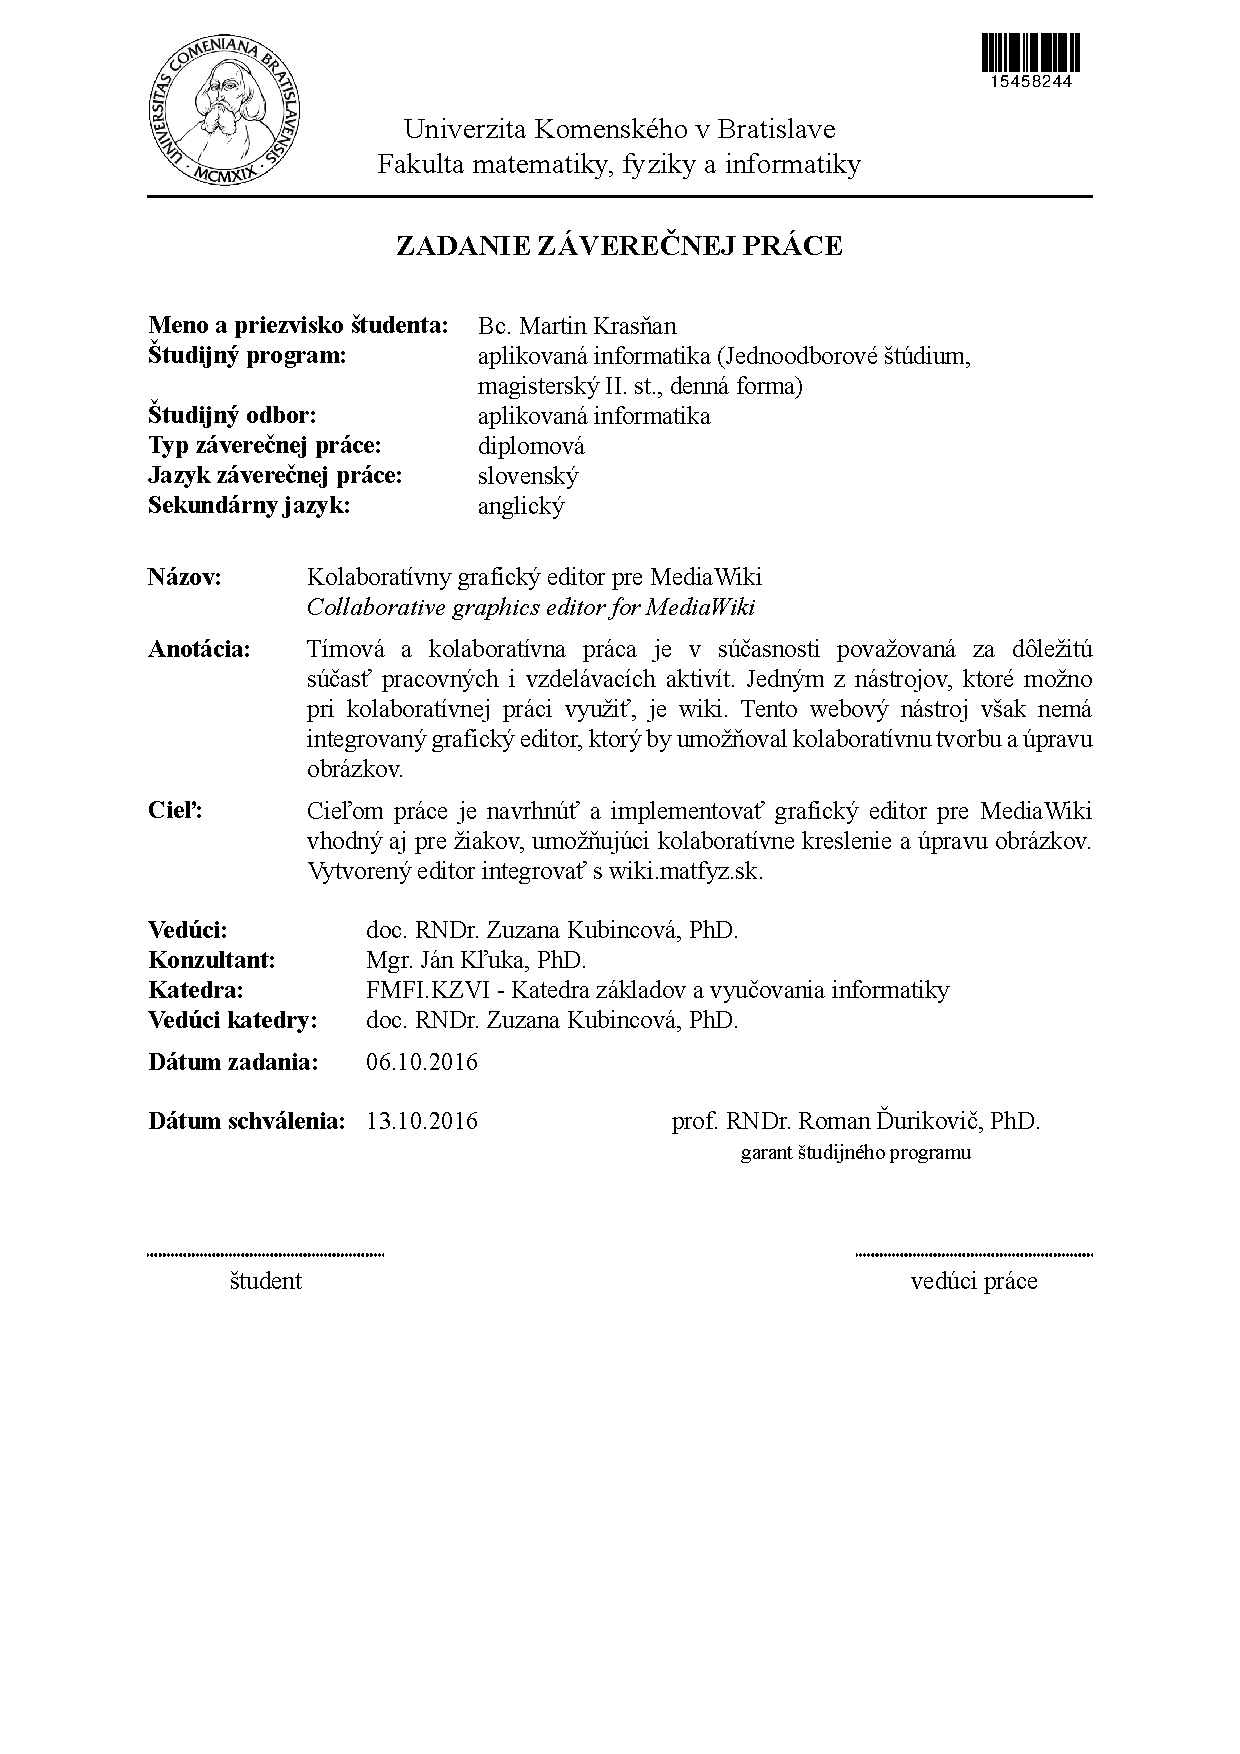
\includegraphics[width=\paperwidth]{images/base/zadaniedp}}
\label{img:zadanie}
\end{center}
\end{figure}

{~}\vspace{12cm}

\noindent
\begin{minipage}{0.25\textwidth}~\end{minipage}
\begin{minipage}{0.75\textwidth}
Čestne vyhlasujem, že som túto diplomovú prácu vypracoval samostatne pod vedením doc. RNDr. Zuzany Kubincovej, PhD., s použitím zdrojov uvedených v zozname použitej literatúry.
\newline \newline
\end{minipage}
\vfill
~ \hfill {\hbox to 6cm{\dotfill}} \\
\mfplacedate \hfill \mfauthor
\vfill\eject 
% koniec prehlasenia

\chapter*{Poďakovanie}\label{chap:thank_you}
...podakovanie...
\vfill\eject 
% koniec podakovania

\chapter*{Abstrakt}\label{chap:abstract_sk}
\MakeUppercase{Krasňan}, Martin: \textit{\mftitle} [\mfthesistype]. - Univerzita Komenského v Bratislave. Fakulta matematiky, fyziky a informatiky; \mfpracovisko. - Školiteľ: \mfadvisor. Bratislava: \mfplacedate. ?? strán.

Text abstraktu...

~\\
Kľúčové slová: klucove, slova, sk, ...
\vfill\eject 

\chapter*{Abstract}\label{chap:abstract_en}
\MakeUppercase{Krasňan}, Martin: \textit{\enmftitle} [\enmfthesistype]. - Comenius University in Bratislava. Faculty of Mathematics, Physics and Informatics; \enmfpracovisko. - Supervisor: \mfadvisor. \mfplacedate. ?? pages.

Text of abstract

~\\
Keywords: keywords, en, ...
\vfill\eject 
% koniec abstraktov



% treba este prejst dokument ci je kod spravne formatovany
\tableofcontents

%zrusenie indentu pre paragraph a nastavenie medzery nad novym riadkom
\def\spaceafterpar{1em}
\setlength{\parskip}{\spaceafterpar}
\setlength\parindent{0pt}

\mainmatter

\input intro.tex
\input motivation.tex
\input issuesoverview.tex
\input previoussolutions.tex
\input proposal.tex
\input implementation.tex
\input results.tex
\input conclusion.tex

\backmatter
\def\spaceafterpar{0em}
\setlength{\parskip}{\spaceafterpar}
\listoffigures

\listoftables



\nocite{*}
\bibliographystyle{alpha}
\bibliography{references}

\end{document}